\documentclass[10pt,letterpaper,landscape]{article}
\usepackage[margin=0.5cm]{geometry}
\usepackage{tikz}
\usetikzlibrary{decorations}
\usetikzlibrary{patterns}

\makeatletter
\@fpsep\textheight
\makeatother


\definecolor{blueprint}{rgb}{0, 0.298, .501}
%\pagecolor{blueprint}
%
%\color{white}
\begin{document}
	\begin{figure}
		\centering
		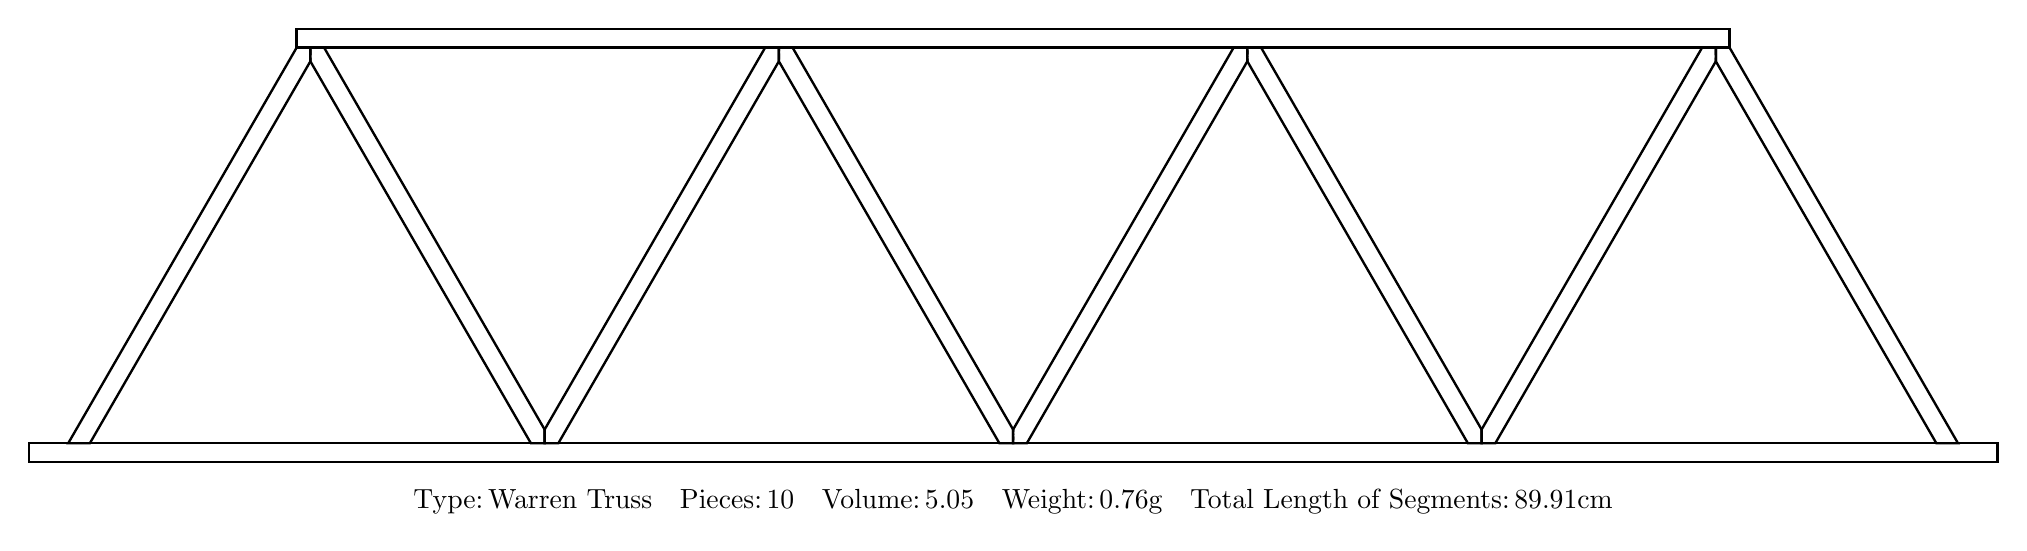
\begin{tikzpicture}
\draw[pattern=crosshatch, pattern color=white, line width=.3mm,] (-0.5,0) -- (24.5,0) -- (24.5,0.238) -- (-0.5,0.238) -- cycle;
\draw[pattern=crosshatch, pattern color=white, line width=.3mm,] (0.27482,0.238) -- (3.07544,5.08882) -- (3.07544,5.26305) -- (2.90121,5.26305) -- (0,0.238) -- cycle;
\draw[pattern=crosshatch, pattern color=white, line width=.3mm,] (23.72518,0.238) -- (20.92456,5.08882) -- (20.92456,5.26305) -- (21.09879,5.26305) -- (24,0.238) -- cycle;
\draw[pattern=crosshatch, pattern color=white, line width=.3mm,] (5.87607,0.238) -- (3.07544,5.08882) -- (3.07544,5.26305) -- (3.24967,5.26305) -- (6.0503,0.41223) -- (6.0503,0.238) -- cycle;
\draw[pattern=crosshatch, pattern color=white, line width=.3mm,] (6.22452,0.238) -- (9.02515,5.08882) -- (9.02515,5.26305) -- (8.85092,5.26305) -- (6.0503,0.41223) -- (6.0503,0.238) -- cycle;
\draw[pattern=crosshatch, pattern color=white, line width=.3mm,] (11.82577,0.238) -- (9.02515,5.08882) -- (9.02515,5.26305) -- (9.19938,5.26305) -- (12,0.41223) -- (12,0.238) -- cycle;
\draw[pattern=crosshatch, pattern color=white, line width=.3mm,] (12.17423,0.238) -- (14.97485,5.08882) -- (14.97485,5.26305) -- (14.80062,5.26305) -- (12,0.41223) -- (12,0.238) -- cycle;
\draw[pattern=crosshatch, pattern color=white, line width=.3mm,] (17.77548,0.238) -- (14.97485,5.08882) -- (14.97485,5.26305) -- (15.14908,5.26305) -- (17.9497,0.41223) -- (17.9497,0.238) -- cycle;
\draw[pattern=crosshatch, pattern color=white, line width=.3mm,] (18.12393,0.238) -- (20.92456,5.08882) -- (20.92456,5.26305) -- (20.75033,5.26305) -- (17.9497,0.41223) -- (17.9497,0.238) -- cycle;
\draw[pattern=crosshatch, pattern color=white, line width=.3mm,] (2.90121,5.26305) -- (21.09879,5.26305) -- (21.09879,5.50105) -- (2.90121,5.50105) -- (2.90121,5.26305) -- cycle;
\path node at (12,-0.5) {Type:\,Warren Truss\quad Pieces:\,10\quad Volume:\,5.05\quad Weight:\,0.76g\quad Total Length of Segments:\,89.91cm};
\end{tikzpicture}

	\end{figure}
	
	\begin{figure}
		\centering
		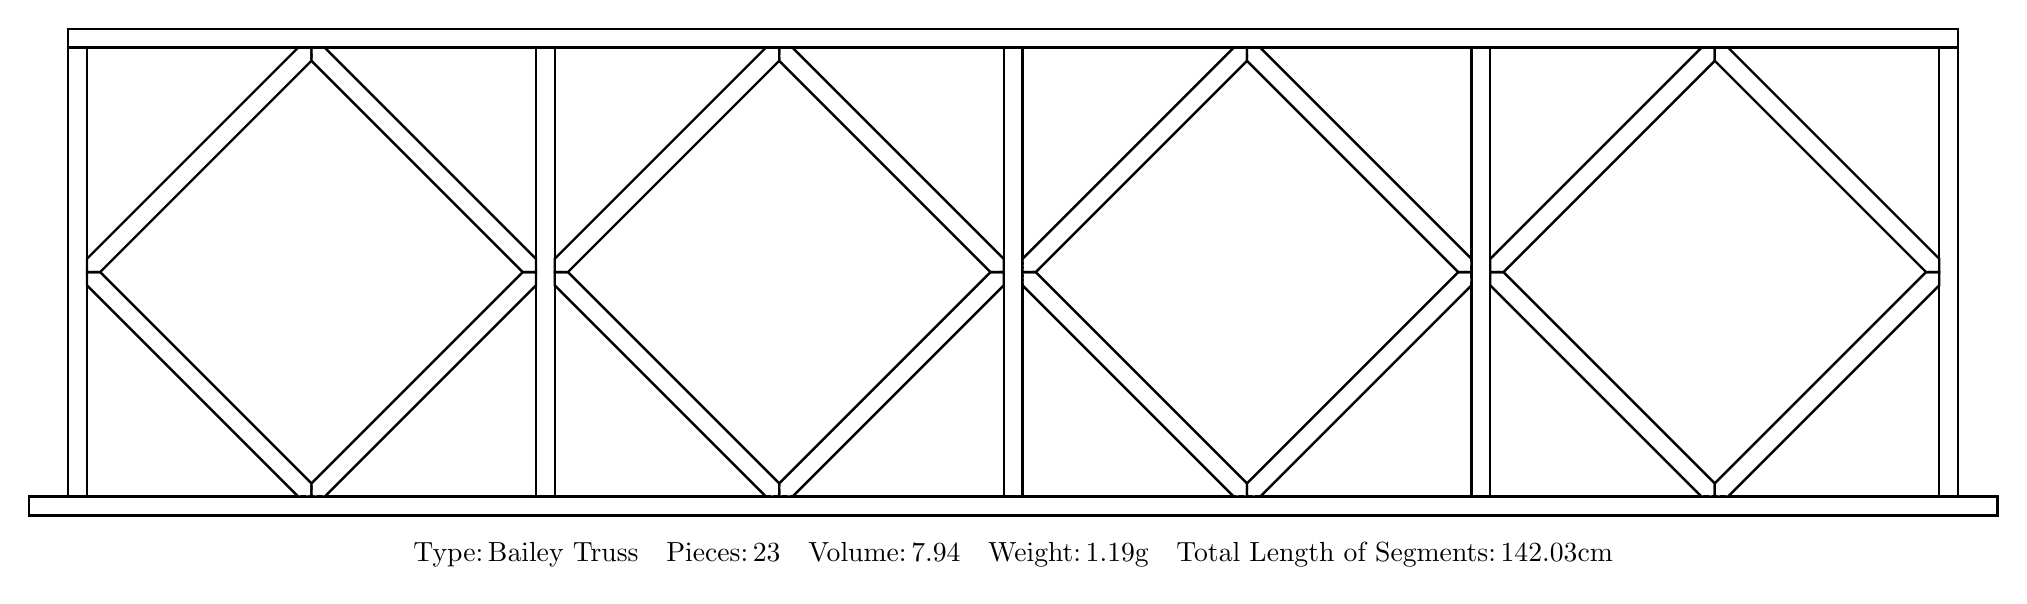
\begin{tikzpicture}
\draw[pattern=crosshatch, pattern color=white, line width=.3mm,] (-0.5,0) -- (24.5,0) -- (24.5,0.238) -- (-0.5,0.238) -- cycle;
\draw[pattern=crosshatch, pattern color=white, line width=.3mm,] (0,0.238) -- (0.238,0.238) -- (0.238,5.9405) -- (0,5.9405) -- cycle;
\draw[pattern=crosshatch, pattern color=white, line width=.3mm,] (5.9405,0.238) -- (6.1785,0.238) -- (6.1785,5.9405) -- (5.9405,5.9405) -- cycle;
\draw[pattern=crosshatch, pattern color=white, line width=.3mm,] (11.881,0.238) -- (12.119,0.238) -- (12.119,5.9405) -- (11.881,5.9405) -- cycle;
\draw[pattern=crosshatch, pattern color=white, line width=.3mm,] (17.8215,0.238) -- (18.0595,0.238) -- (18.0595,5.9405) -- (17.8215,5.9405) -- cycle;
\draw[pattern=crosshatch, pattern color=white, line width=.3mm,] (23.762,0.238) -- (24,0.238) -- (24,5.9405) -- (23.762,5.9405) -- cycle;
\draw[pattern=crosshatch, pattern color=white, line width=.3mm,] (2.92096,0.238) -- (0.238,2.92096) -- (0.238,3.08925) -- (0.40629,3.08925) -- (3.08925,0.40629) -- (3.08925,0.238) -- cycle;
\draw[pattern=crosshatch, pattern color=white, line width=.3mm,] (3.25754,0.238) -- (5.9405,2.92096) -- (5.9405,3.08925) -- (5.77221,3.08925) -- (3.08925,0.40629) -- (3.08925,0.238) -- cycle;
\draw[pattern=crosshatch, pattern color=white, line width=.3mm,] (2.92096,5.9405) -- (0.238,3.25754) -- (0.238,3.08925) -- (0.40629,3.08925) -- (3.08925,5.77221) -- (3.08925,5.9405) -- cycle;
\draw[pattern=crosshatch, pattern color=white, line width=.3mm,] (3.25754,5.9405) -- (5.9405,3.25754) -- (5.9405,3.08925) -- (5.77221,3.08925) -- (3.08925,5.77221) -- (3.08925,5.9405) -- cycle;
\draw[pattern=crosshatch, pattern color=white, line width=.3mm,] (8.86146,0.238) -- (6.1785,2.92096) -- (6.1785,3.08925) -- (6.34679,3.08925) -- (9.02975,0.40629) -- (9.02975,0.238) -- cycle;
\draw[pattern=crosshatch, pattern color=white, line width=.3mm,] (9.19804,0.238) -- (11.881,2.92096) -- (11.881,3.08925) -- (11.71271,3.08925) -- (9.02975,0.40629) -- (9.02975,0.238) -- cycle;
\draw[pattern=crosshatch, pattern color=white, line width=.3mm,] (8.86146,5.9405) -- (6.1785,3.25754) -- (6.1785,3.08925) -- (6.34679,3.08925) -- (9.02975,5.77221) -- (9.02975,5.9405) -- cycle;
\draw[pattern=crosshatch, pattern color=white, line width=.3mm,] (9.19804,5.9405) -- (11.881,3.25754) -- (11.881,3.08925) -- (11.71271,3.08925) -- (9.02975,5.77221) -- (9.02975,5.9405) -- cycle;
\draw[pattern=crosshatch, pattern color=white, line width=.3mm,] (14.80196,0.238) -- (12.119,2.92096) -- (12.119,3.08925) -- (12.28729,3.08925) -- (14.97025,0.40629) -- (14.97025,0.238) -- cycle;
\draw[pattern=crosshatch, pattern color=white, line width=.3mm,] (15.13854,0.238) -- (17.8215,2.92096) -- (17.8215,3.08925) -- (17.65321,3.08925) -- (14.97025,0.40629) -- (14.97025,0.238) -- cycle;
\draw[pattern=crosshatch, pattern color=white, line width=.3mm,] (14.80196,5.9405) -- (12.119,3.25754) -- (12.119,3.08925) -- (12.28729,3.08925) -- (14.97025,5.77221) -- (14.97025,5.9405) -- cycle;
\draw[pattern=crosshatch, pattern color=white, line width=.3mm,] (15.13854,5.9405) -- (17.8215,3.25754) -- (17.8215,3.08925) -- (17.65321,3.08925) -- (14.97025,5.77221) -- (14.97025,5.9405) -- cycle;
\draw[pattern=crosshatch, pattern color=white, line width=.3mm,] (20.74246,0.238) -- (18.0595,2.92096) -- (18.0595,3.08925) -- (18.22779,3.08925) -- (20.91075,0.40629) -- (20.91075,0.238) -- cycle;
\draw[pattern=crosshatch, pattern color=white, line width=.3mm,] (21.07904,0.238) -- (23.762,2.92096) -- (23.762,3.08925) -- (23.59371,3.08925) -- (20.91075,0.40629) -- (20.91075,0.238) -- cycle;
\draw[pattern=crosshatch, pattern color=white, line width=.3mm,] (20.74246,5.9405) -- (18.0595,3.25754) -- (18.0595,3.08925) -- (18.22779,3.08925) -- (20.91075,5.77221) -- (20.91075,5.9405) -- cycle;
\draw[pattern=crosshatch, pattern color=white, line width=.3mm,] (21.07904,5.9405) -- (23.762,3.25754) -- (23.762,3.08925) -- (23.59371,3.08925) -- (20.91075,5.77221) -- (20.91075,5.9405) -- cycle;
\draw[pattern=crosshatch, pattern color=white, line width=.3mm,] (0,5.9405) -- (24,5.9405) -- (24,6.1785) -- (0,6.1785) -- (0,5.9405) -- cycle;
\path node at (12,-0.5) {Type:\,Bailey Truss\quad Pieces:\,23\quad Volume:\,7.94\quad Weight:\,1.19g\quad Total Length of Segments:\,142.03cm};
\end{tikzpicture}

	\end{figure}
	\begin{figure}
		\centering
		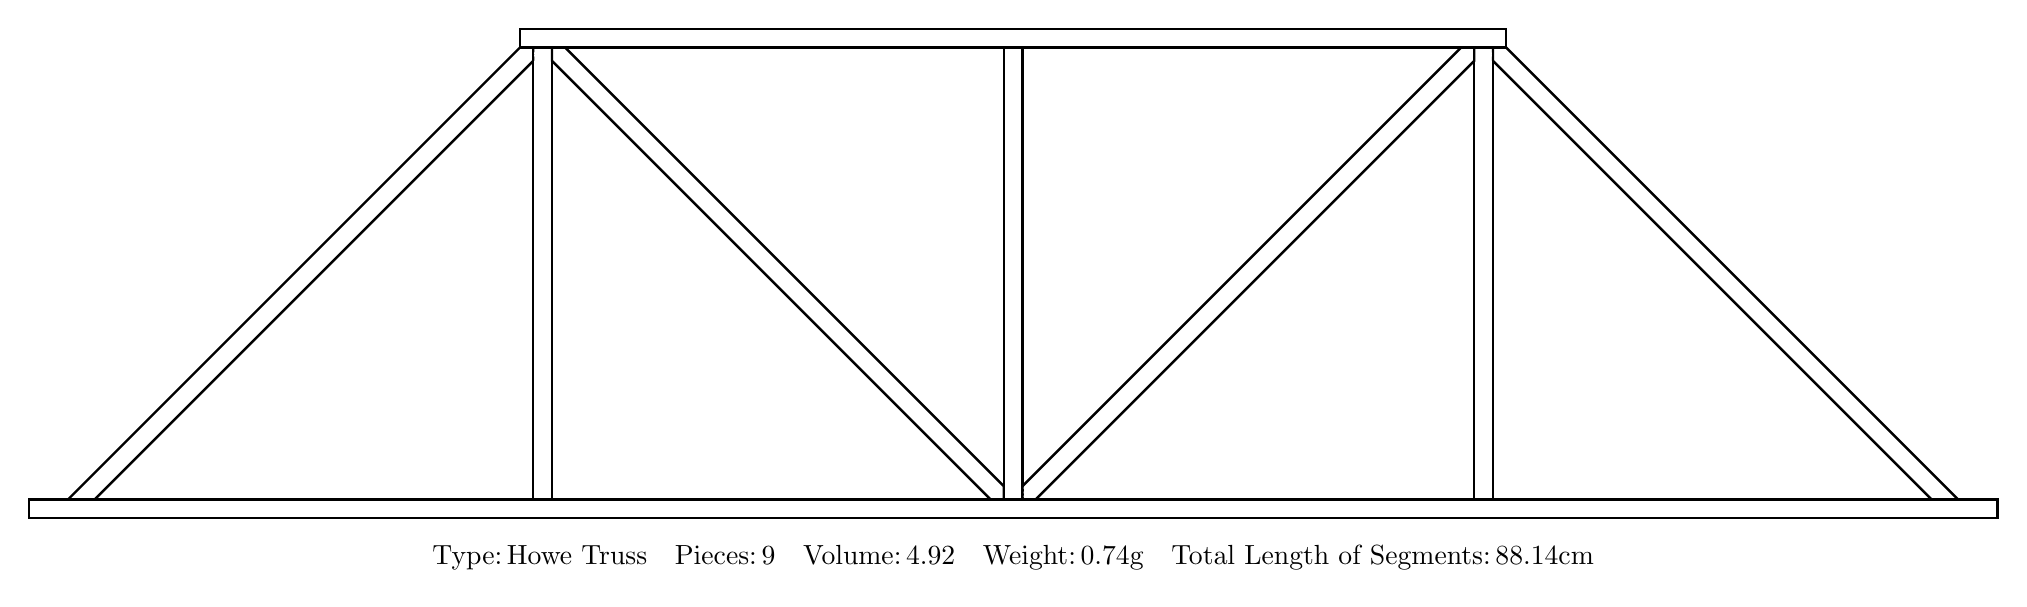
\begin{tikzpicture}
\draw[pattern=crosshatch, pattern color=white, line width=.3mm,] (-0.5,0) -- (24.5,0) -- (24.5,0.238) -- (-0.5,0.238) -- cycle;
\draw[pattern=crosshatch, pattern color=white, line width=.3mm,] (0,0.238) -- (5.73735,5.97535) -- (5.90565,5.97535) -- (5.90565,5.80706) -- (0.33658,0.238) -- cycle;
\draw[pattern=crosshatch, pattern color=white, line width=.3mm,] (24,0.238) -- (18.26265,5.97535) -- (18.09435,5.97535) -- (18.09435,5.80706) -- (23.66342,0.238) -- cycle;
\draw[pattern=crosshatch, pattern color=white, line width=.3mm,] (5.90565,0.238) -- (5.90565,5.97535) -- (6.14365,5.97535) -- (6.14365,0.238) -- cycle;
\draw[pattern=crosshatch, pattern color=white, line width=.3mm,] (11.881,0.238) -- (11.881,5.97535) -- (12.119,5.97535) -- (12.119,0.238) -- cycle;
\draw[pattern=crosshatch, pattern color=white, line width=.3mm,] (17.85635,0.238) -- (17.85635,5.97535) -- (18.09435,5.97535) -- (18.09435,0.238) -- cycle;
\draw[pattern=crosshatch, pattern color=white, line width=.3mm,] (12.28729,0.238) -- (17.85635,5.80706) -- (17.85635,5.97535) -- (17.68806,5.97535) -- (12.119,0.40629) -- (12.119,0.238) -- cycle;
\draw[pattern=crosshatch, pattern color=white, line width=.3mm,] (11.71271,0.238) -- (6.14365,5.80706) -- (6.14365,5.97535) -- (6.31194,5.97535) -- (11.881,0.40629) -- (11.881,0.238) -- cycle;
\draw[pattern=crosshatch, pattern color=white, line width=.3mm,] (5.73735,5.97535) -- (18.26265,5.97535) -- (18.26265,6.21335) -- (5.73735,6.21335) -- cycle;
\path node at (12,-0.5) {Type:\,Howe Truss\quad Pieces:\,9\quad Volume:\,4.92\quad Weight:\,0.74g\quad Total Length of Segments:\,88.14cm};
\end{tikzpicture}

	\end{figure}
	\begin{figure}
		\centering
		\input{latexbridges/figures/pratt4.tex}
	\end{figure}
	\begin{figure}
		\centering
		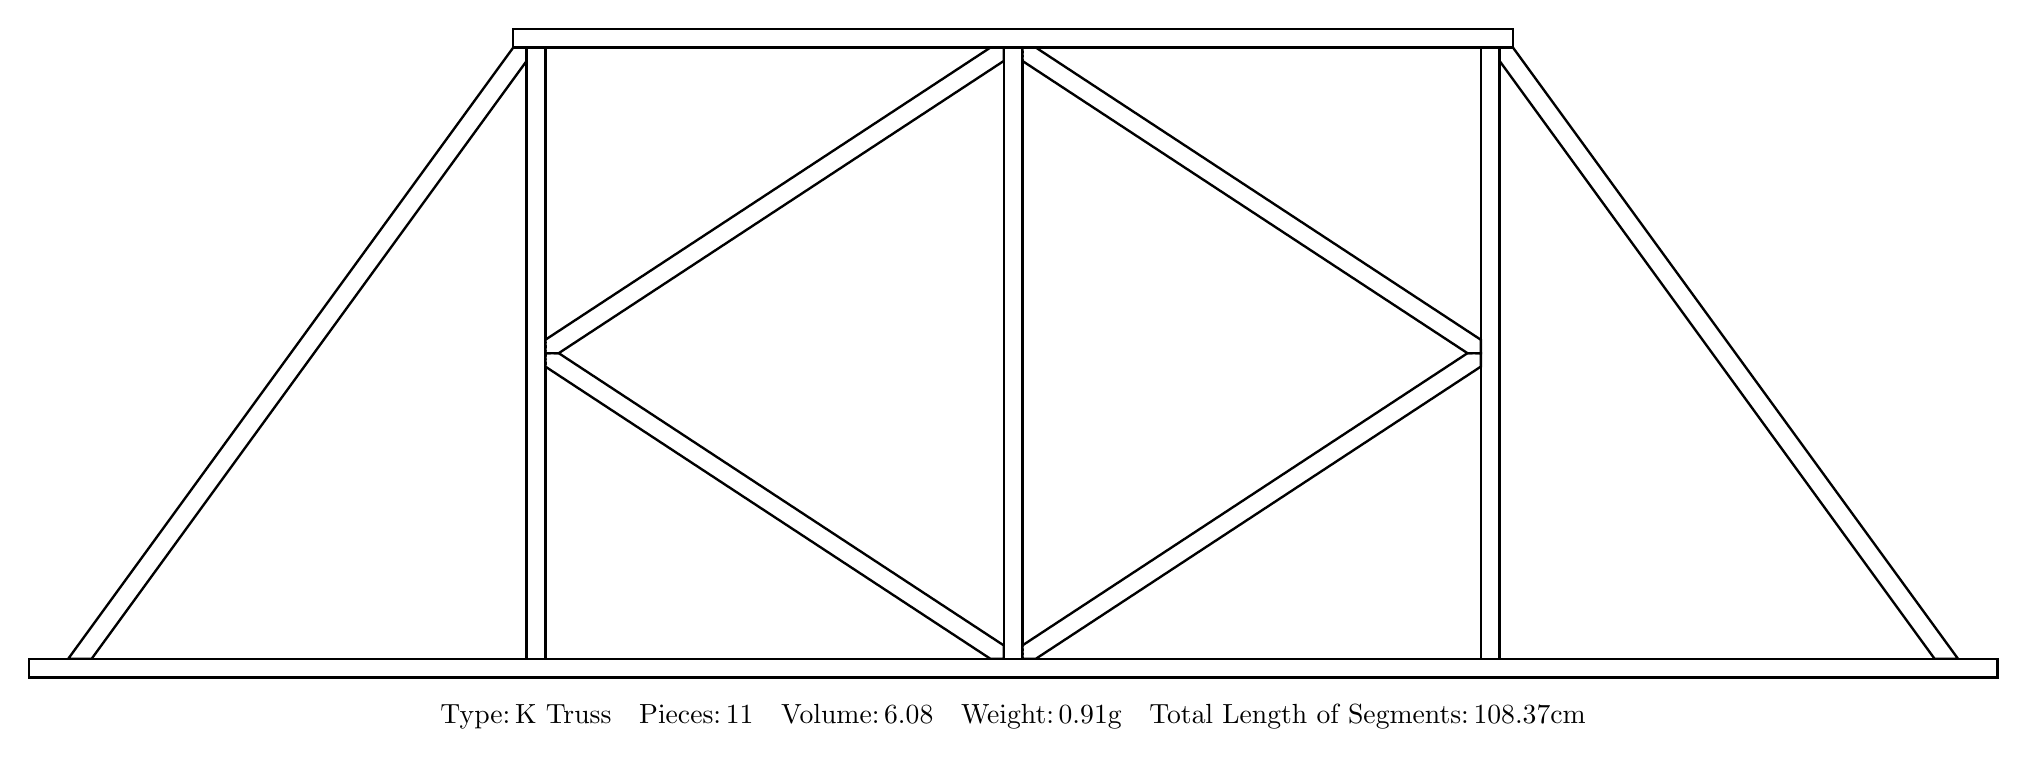
\begin{tikzpicture}
\draw[pattern=crosshatch, pattern color=white, line width=.3mm,] (-0.5,0) -- (24.5,0) -- (24.5,0.238) -- (-0.5,0.238) -- cycle;
\draw[pattern=crosshatch, pattern color=white, line width=.3mm,] (0,0.238) -- (0.2975,0.238) -- (5.8215,7.83) -- (5.8215,8) -- (5.6515,8) -- cycle;
\draw[pattern=crosshatch, pattern color=white, line width=.3mm,] (24,0.238) -- (23.7025,0.238) -- (18.1785,7.83) -- (18.1785,8) -- (18.3485,8) -- cycle;
\draw[pattern=crosshatch, pattern color=white, line width=.3mm,] (5.8215,0.238) -- (5.8215,8) -- (6.0595,8) -- (6.0595,0.238) -- cycle;
\draw[pattern=crosshatch, pattern color=white, line width=.3mm,] (11.881,0.238) -- (11.881,8) -- (12.119,8) -- (12.119,0.238) -- cycle;
\draw[pattern=crosshatch, pattern color=white, line width=.3mm,] (17.9405,0.238) -- (17.9405,8) -- (18.1785,8) -- (18.1785,0.238) -- cycle;
\draw[pattern=crosshatch, pattern color=white, line width=.3mm,] (6.0595,4.119) -- (6.22959,4.119) -- (11.881,7.82991) -- (11.881,8) -- (11.71091,8) -- (6.0595,4.28909) -- cycle;
\draw[pattern=crosshatch, pattern color=white, line width=.3mm,] (6.0595,4.119) -- (6.0595,3.94891) -- (11.71091,0.238) -- (11.881,0.238) -- (11.881,0.40809) -- (6.22959,4.119) -- cycle;
\draw[pattern=crosshatch, pattern color=white, line width=.3mm,] (17.9405,4.119) -- (17.77041,4.119) -- (12.119,7.82991) -- (12.119,8) -- (12.28909,8) -- (17.9405,4.28909) -- cycle;
\draw[pattern=crosshatch, pattern color=white, line width=.3mm,] (17.9405,4.119) -- (17.9405,3.94891) -- (12.28909,0.238) -- (12.119,0.238) -- (12.119,0.40809) -- (17.77041,4.119) -- cycle;
\draw[pattern=crosshatch, pattern color=white, line width=.3mm,] (5.6515,8) -- (18.3485,8) -- (18.3485,8.238) -- (5.6515,8.238) -- cycle;
\path node at (12,-0.5) {Type:\,K Truss\quad Pieces:\,11\quad Volume:\,6.08\quad Weight:\,0.91g\quad Total Length of Segments:\,108.37cm};
\end{tikzpicture}

	\end{figure}
	\begin{figure}
		\centering
		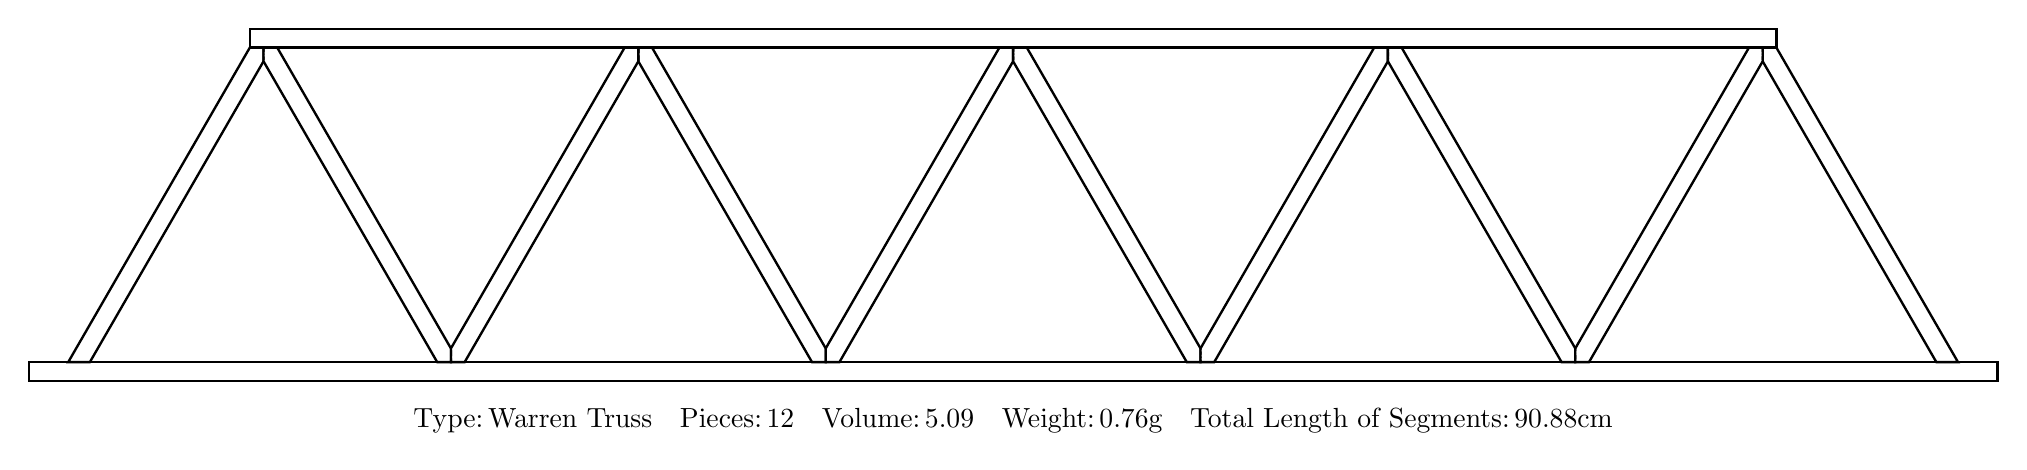
\begin{tikzpicture}
\draw[pattern=crosshatch, pattern color=white, line width=.3mm,] (-0.5,0) -- (24.5,0) -- (24.5,0.238) -- (-0.5,0.238) -- cycle;
\draw[pattern=crosshatch, pattern color=white, line width=.3mm,] (0.27482,0.238) -- (2.48047,4.0583) -- (2.48047,4.23253) -- (2.30624,4.23253) -- (0,0.238) -- cycle;
\draw[pattern=crosshatch, pattern color=white, line width=.3mm,] (23.72518,0.238) -- (21.51953,4.0583) -- (21.51953,4.23253) -- (21.69376,4.23253) -- (24,0.238) -- cycle;
\draw[pattern=crosshatch, pattern color=white, line width=.3mm,] (4.68613,0.238) -- (2.48047,4.0583) -- (2.48047,4.23253) -- (2.6547,4.23253) -- (4.86035,0.41223) -- (4.86035,0.238) -- cycle;
\draw[pattern=crosshatch, pattern color=white, line width=.3mm,] (5.03458,0.238) -- (7.24024,4.0583) -- (7.24024,4.23253) -- (7.06601,4.23253) -- (4.86035,0.41223) -- (4.86035,0.238) -- cycle;
\draw[pattern=crosshatch, pattern color=white, line width=.3mm,] (9.44589,0.238) -- (7.24024,4.0583) -- (7.24024,4.23253) -- (7.41446,4.23253) -- (9.62012,0.41223) -- (9.62012,0.238) -- cycle;
\draw[pattern=crosshatch, pattern color=white, line width=.3mm,] (9.79435,0.238) -- (12,4.0583) -- (12,4.23253) -- (11.82577,4.23253) -- (9.62012,0.41223) -- (9.62012,0.238) -- cycle;
\draw[pattern=crosshatch, pattern color=white, line width=.3mm,] (14.20565,0.238) -- (12,4.0583) -- (12,4.23253) -- (12.17423,4.23253) -- (14.37988,0.41223) -- (14.37988,0.238) -- cycle;
\draw[pattern=crosshatch, pattern color=white, line width=.3mm,] (14.55411,0.238) -- (16.75976,4.0583) -- (16.75976,4.23253) -- (16.58554,4.23253) -- (14.37988,0.41223) -- (14.37988,0.238) -- cycle;
\draw[pattern=crosshatch, pattern color=white, line width=.3mm,] (18.96542,0.238) -- (16.75976,4.0583) -- (16.75976,4.23253) -- (16.93399,4.23253) -- (19.13965,0.41223) -- (19.13965,0.238) -- cycle;
\draw[pattern=crosshatch, pattern color=white, line width=.3mm,] (19.31387,0.238) -- (21.51953,4.0583) -- (21.51953,4.23253) -- (21.3453,4.23253) -- (19.13965,0.41223) -- (19.13965,0.238) -- cycle;
\draw[pattern=crosshatch, pattern color=white, line width=.3mm,] (2.30624,4.23253) -- (21.69376,4.23253) -- (21.69376,4.47053) -- (2.30624,4.47053) -- (2.30624,4.23253) -- cycle;
\path node at (12,-0.5) {Type:\,Warren Truss\quad Pieces:\,12\quad Volume:\,5.09\quad Weight:\,0.76g\quad Total Length of Segments:\,90.88cm};
\end{tikzpicture}

	\end{figure}
	\begin{figure}
		\centering
		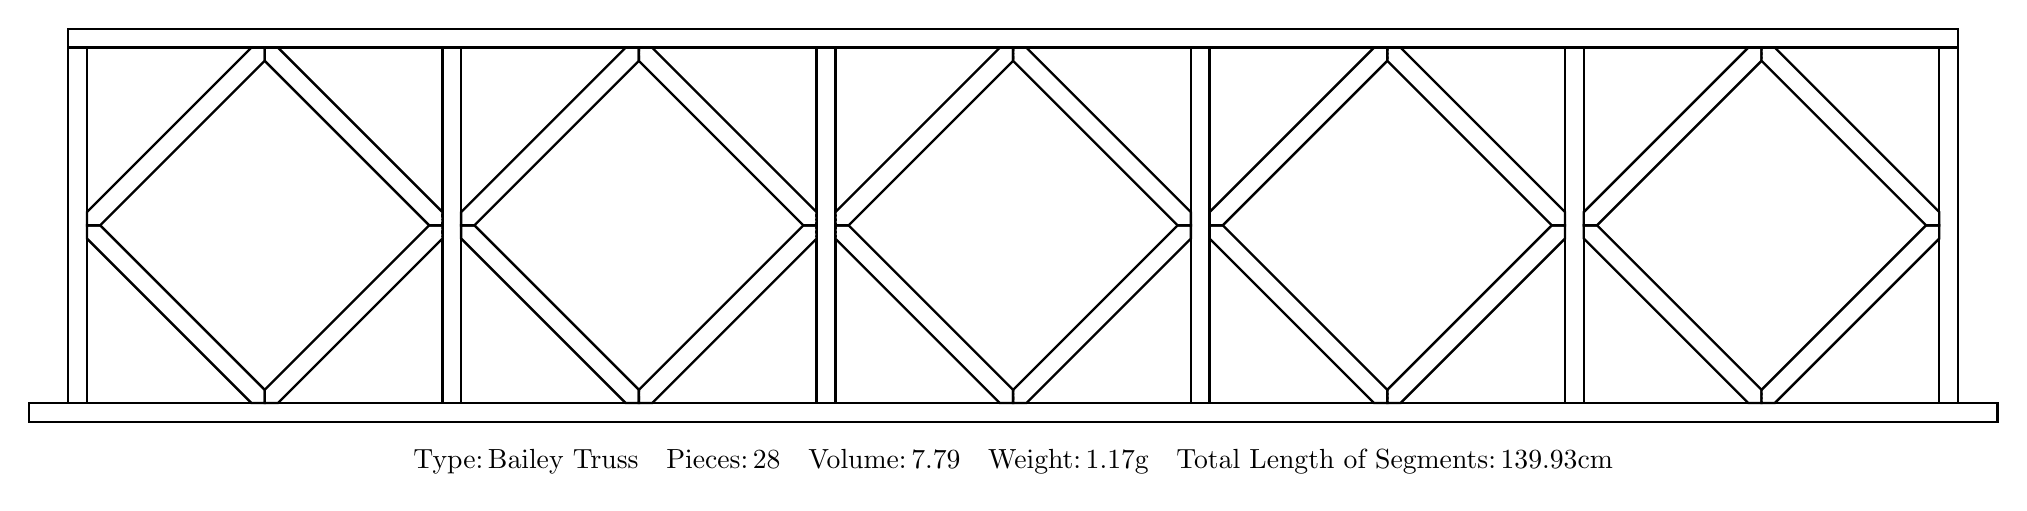
\begin{tikzpicture}
\draw[pattern=crosshatch, pattern color=white, line width=.3mm,] (-0.5,0) -- (24.5,0) -- (24.5,0.238) -- (-0.5,0.238) -- cycle;
\draw[pattern=crosshatch, pattern color=white, line width=.3mm,] (0,0.238) -- (0.238,0.238) -- (0.238,4.7524) -- (0,4.7524) -- cycle;
\draw[pattern=crosshatch, pattern color=white, line width=.3mm,] (4.7524,0.238) -- (4.9904,0.238) -- (4.9904,4.7524) -- (4.7524,4.7524) -- cycle;
\draw[pattern=crosshatch, pattern color=white, line width=.3mm,] (9.5048,0.238) -- (9.7428,0.238) -- (9.7428,4.7524) -- (9.5048,4.7524) -- cycle;
\draw[pattern=crosshatch, pattern color=white, line width=.3mm,] (14.2572,0.238) -- (14.4952,0.238) -- (14.4952,4.7524) -- (14.2572,4.7524) -- cycle;
\draw[pattern=crosshatch, pattern color=white, line width=.3mm,] (19.0096,0.238) -- (19.2476,0.238) -- (19.2476,4.7524) -- (19.0096,4.7524) -- cycle;
\draw[pattern=crosshatch, pattern color=white, line width=.3mm,] (23.762,0.238) -- (24,0.238) -- (24,4.7524) -- (23.762,4.7524) -- cycle;
\draw[pattern=crosshatch, pattern color=white, line width=.3mm,] (2.32691,0.238) -- (0.238,2.32691) -- (0.238,2.4952) -- (0.40629,2.4952) -- (2.4952,0.40629) -- (2.4952,0.238) -- cycle;
\draw[pattern=crosshatch, pattern color=white, line width=.3mm,] (2.66349,0.238) -- (4.7524,2.32691) -- (4.7524,2.4952) -- (4.58411,2.4952) -- (2.4952,0.40629) -- (2.4952,0.238) -- cycle;
\draw[pattern=crosshatch, pattern color=white, line width=.3mm,] (2.32691,4.7524) -- (0.238,2.66349) -- (0.238,2.4952) -- (0.40629,2.4952) -- (2.4952,4.58411) -- (2.4952,4.7524) -- cycle;
\draw[pattern=crosshatch, pattern color=white, line width=.3mm,] (2.66349,4.7524) -- (4.7524,2.66349) -- (4.7524,2.4952) -- (4.58411,2.4952) -- (2.4952,4.58411) -- (2.4952,4.7524) -- cycle;
\draw[pattern=crosshatch, pattern color=white, line width=.3mm,] (7.07931,0.238) -- (4.9904,2.32691) -- (4.9904,2.4952) -- (5.15869,2.4952) -- (7.2476,0.40629) -- (7.2476,0.238) -- cycle;
\draw[pattern=crosshatch, pattern color=white, line width=.3mm,] (7.41589,0.238) -- (9.5048,2.32691) -- (9.5048,2.4952) -- (9.33651,2.4952) -- (7.2476,0.40629) -- (7.2476,0.238) -- cycle;
\draw[pattern=crosshatch, pattern color=white, line width=.3mm,] (7.07931,4.7524) -- (4.9904,2.66349) -- (4.9904,2.4952) -- (5.15869,2.4952) -- (7.2476,4.58411) -- (7.2476,4.7524) -- cycle;
\draw[pattern=crosshatch, pattern color=white, line width=.3mm,] (7.41589,4.7524) -- (9.5048,2.66349) -- (9.5048,2.4952) -- (9.33651,2.4952) -- (7.2476,4.58411) -- (7.2476,4.7524) -- cycle;
\draw[pattern=crosshatch, pattern color=white, line width=.3mm,] (11.83171,0.238) -- (9.7428,2.32691) -- (9.7428,2.4952) -- (9.91109,2.4952) -- (12,0.40629) -- (12,0.238) -- cycle;
\draw[pattern=crosshatch, pattern color=white, line width=.3mm,] (12.16829,0.238) -- (14.2572,2.32691) -- (14.2572,2.4952) -- (14.08891,2.4952) -- (12,0.40629) -- (12,0.238) -- cycle;
\draw[pattern=crosshatch, pattern color=white, line width=.3mm,] (11.83171,4.7524) -- (9.7428,2.66349) -- (9.7428,2.4952) -- (9.91109,2.4952) -- (12,4.58411) -- (12,4.7524) -- cycle;
\draw[pattern=crosshatch, pattern color=white, line width=.3mm,] (12.16829,4.7524) -- (14.2572,2.66349) -- (14.2572,2.4952) -- (14.08891,2.4952) -- (12,4.58411) -- (12,4.7524) -- cycle;
\draw[pattern=crosshatch, pattern color=white, line width=.3mm,] (16.58411,0.238) -- (14.4952,2.32691) -- (14.4952,2.4952) -- (14.66349,2.4952) -- (16.7524,0.40629) -- (16.7524,0.238) -- cycle;
\draw[pattern=crosshatch, pattern color=white, line width=.3mm,] (16.92069,0.238) -- (19.0096,2.32691) -- (19.0096,2.4952) -- (18.84131,2.4952) -- (16.7524,0.40629) -- (16.7524,0.238) -- cycle;
\draw[pattern=crosshatch, pattern color=white, line width=.3mm,] (16.58411,4.7524) -- (14.4952,2.66349) -- (14.4952,2.4952) -- (14.66349,2.4952) -- (16.7524,4.58411) -- (16.7524,4.7524) -- cycle;
\draw[pattern=crosshatch, pattern color=white, line width=.3mm,] (16.92069,4.7524) -- (19.0096,2.66349) -- (19.0096,2.4952) -- (18.84131,2.4952) -- (16.7524,4.58411) -- (16.7524,4.7524) -- cycle;
\draw[pattern=crosshatch, pattern color=white, line width=.3mm,] (21.33651,0.238) -- (19.2476,2.32691) -- (19.2476,2.4952) -- (19.41589,2.4952) -- (21.5048,0.40629) -- (21.5048,0.238) -- cycle;
\draw[pattern=crosshatch, pattern color=white, line width=.3mm,] (21.67309,0.238) -- (23.762,2.32691) -- (23.762,2.4952) -- (23.59371,2.4952) -- (21.5048,0.40629) -- (21.5048,0.238) -- cycle;
\draw[pattern=crosshatch, pattern color=white, line width=.3mm,] (21.33651,4.7524) -- (19.2476,2.66349) -- (19.2476,2.4952) -- (19.41589,2.4952) -- (21.5048,4.58411) -- (21.5048,4.7524) -- cycle;
\draw[pattern=crosshatch, pattern color=white, line width=.3mm,] (21.67309,4.7524) -- (23.762,2.66349) -- (23.762,2.4952) -- (23.59371,2.4952) -- (21.5048,4.58411) -- (21.5048,4.7524) -- cycle;
\draw[pattern=crosshatch, pattern color=white, line width=.3mm,] (0,4.7524) -- (24,4.7524) -- (24,4.9904) -- (0,4.9904) -- (0,4.7524) -- cycle;
\path node at (12,-0.5) {Type:\,Bailey Truss\quad Pieces:\,28\quad Volume:\,7.79\quad Weight:\,1.17g\quad Total Length of Segments:\,139.93cm};
\end{tikzpicture}

	\end{figure}
	\begin{figure}
		\centering
		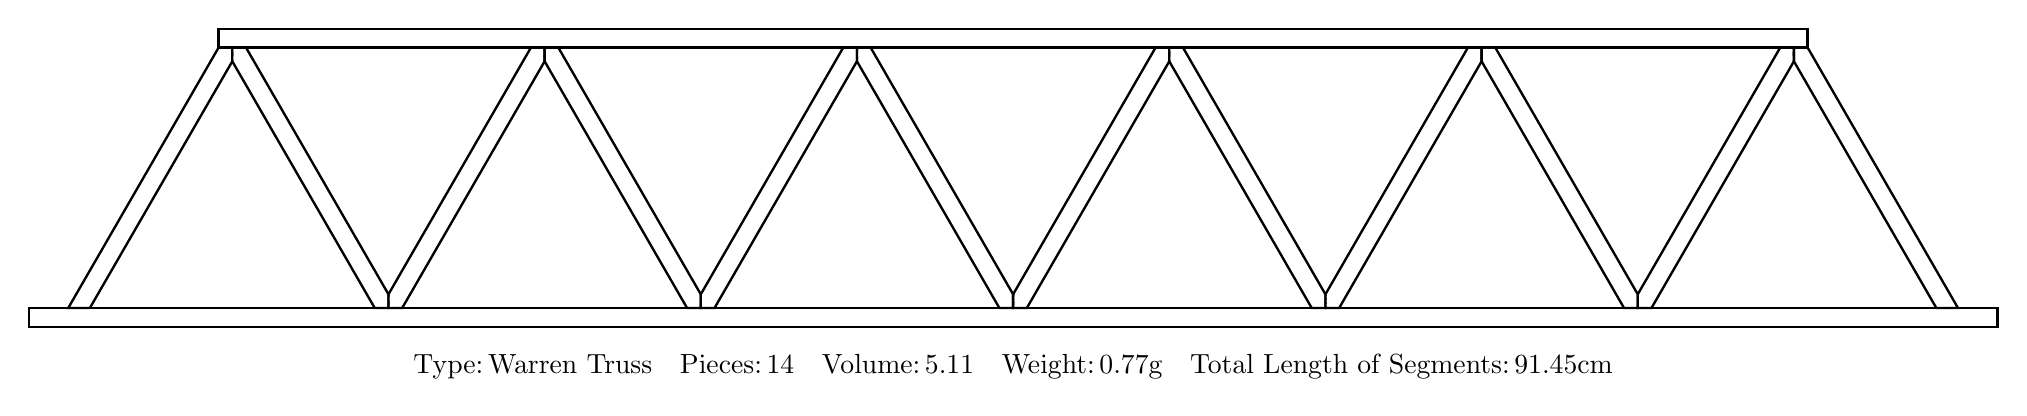
\begin{tikzpicture}
\draw[pattern=crosshatch, pattern color=white, line width=.3mm,] (-0.5,0) -- (24.5,0) -- (24.5,0.238) -- (-0.5,0.238) -- cycle;
\draw[pattern=crosshatch, pattern color=white, line width=.3mm,] (0.27482,0.238) -- (2.08383,3.37129) -- (2.08383,3.54552) -- (1.9096,3.54552) -- (0,0.238) -- cycle;
\draw[pattern=crosshatch, pattern color=white, line width=.3mm,] (23.72518,0.238) -- (21.91617,3.37129) -- (21.91617,3.54552) -- (22.0904,3.54552) -- (24,0.238) -- cycle;
\draw[pattern=crosshatch, pattern color=white, line width=.3mm,] (3.89283,0.238) -- (2.08383,3.37129) -- (2.08383,3.54552) -- (2.25805,3.54552) -- (4.06706,0.41223) -- (4.06706,0.238) -- cycle;
\draw[pattern=crosshatch, pattern color=white, line width=.3mm,] (4.24129,0.238) -- (6.0503,3.37129) -- (6.0503,3.54552) -- (5.87607,3.54552) -- (4.06706,0.41223) -- (4.06706,0.238) -- cycle;
\draw[pattern=crosshatch, pattern color=white, line width=.3mm,] (7.8593,0.238) -- (6.0503,3.37129) -- (6.0503,3.54552) -- (6.22452,3.54552) -- (8.03353,0.41223) -- (8.03353,0.238) -- cycle;
\draw[pattern=crosshatch, pattern color=white, line width=.3mm,] (8.20776,0.238) -- (10.01677,3.37129) -- (10.01677,3.54552) -- (9.84254,3.54552) -- (8.03353,0.41223) -- (8.03353,0.238) -- cycle;
\draw[pattern=crosshatch, pattern color=white, line width=.3mm,] (11.82577,0.238) -- (10.01677,3.37129) -- (10.01677,3.54552) -- (10.19099,3.54552) -- (12,0.41223) -- (12,0.238) -- cycle;
\draw[pattern=crosshatch, pattern color=white, line width=.3mm,] (12.17423,0.238) -- (13.98323,3.37129) -- (13.98323,3.54552) -- (13.80901,3.54552) -- (12,0.41223) -- (12,0.238) -- cycle;
\draw[pattern=crosshatch, pattern color=white, line width=.3mm,] (15.79224,0.238) -- (13.98323,3.37129) -- (13.98323,3.54552) -- (14.15746,3.54552) -- (15.96647,0.41223) -- (15.96647,0.238) -- cycle;
\draw[pattern=crosshatch, pattern color=white, line width=.3mm,] (16.1407,0.238) -- (17.9497,3.37129) -- (17.9497,3.54552) -- (17.77548,3.54552) -- (15.96647,0.41223) -- (15.96647,0.238) -- cycle;
\draw[pattern=crosshatch, pattern color=white, line width=.3mm,] (19.75871,0.238) -- (17.9497,3.37129) -- (17.9497,3.54552) -- (18.12393,3.54552) -- (19.93294,0.41223) -- (19.93294,0.238) -- cycle;
\draw[pattern=crosshatch, pattern color=white, line width=.3mm,] (20.10717,0.238) -- (21.91617,3.37129) -- (21.91617,3.54552) -- (21.74195,3.54552) -- (19.93294,0.41223) -- (19.93294,0.238) -- cycle;
\draw[pattern=crosshatch, pattern color=white, line width=.3mm,] (1.9096,3.54552) -- (22.0904,3.54552) -- (22.0904,3.78352) -- (1.9096,3.78352) -- (1.9096,3.54552) -- cycle;
\path node at (12,-0.5) {Type:\,Warren Truss\quad Pieces:\,14\quad Volume:\,5.11\quad Weight:\,0.77g\quad Total Length of Segments:\,91.45cm};
\end{tikzpicture}

	\end{figure}
	\begin{figure}
		\centering
		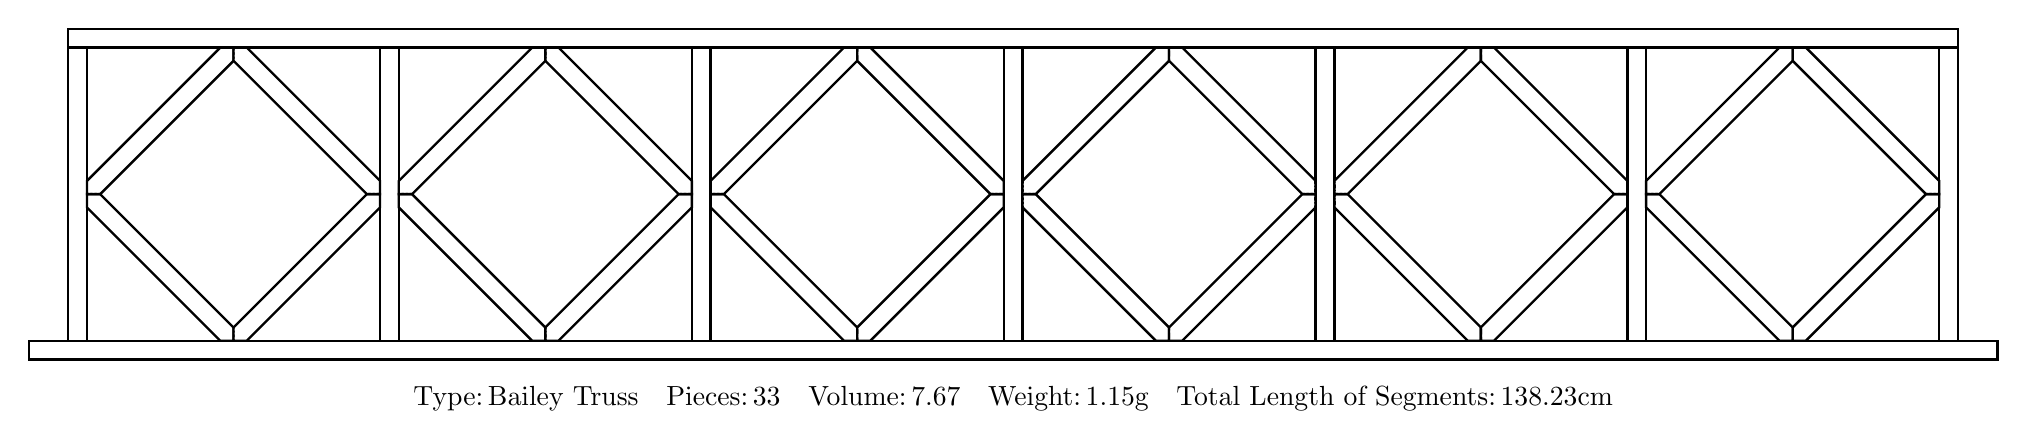
\begin{tikzpicture}
\draw[pattern=crosshatch, pattern color=white, line width=.3mm,] (-0.5,0) -- (24.5,0) -- (24.5,0.238) -- (-0.5,0.238) -- cycle;
\draw[pattern=crosshatch, pattern color=white, line width=.3mm,] (0,0.238) -- (0.238,0.238) -- (0.238,3.96033) -- (0,3.96033) -- cycle;
\draw[pattern=crosshatch, pattern color=white, line width=.3mm,] (3.96033,0.238) -- (4.19833,0.238) -- (4.19833,3.96033) -- (3.96033,3.96033) -- cycle;
\draw[pattern=crosshatch, pattern color=white, line width=.3mm,] (7.92067,0.238) -- (8.15867,0.238) -- (8.15867,3.96033) -- (7.92067,3.96033) -- cycle;
\draw[pattern=crosshatch, pattern color=white, line width=.3mm,] (11.881,0.238) -- (12.119,0.238) -- (12.119,3.96033) -- (11.881,3.96033) -- cycle;
\draw[pattern=crosshatch, pattern color=white, line width=.3mm,] (15.84133,0.238) -- (16.07933,0.238) -- (16.07933,3.96033) -- (15.84133,3.96033) -- cycle;
\draw[pattern=crosshatch, pattern color=white, line width=.3mm,] (19.80167,0.238) -- (20.03967,0.238) -- (20.03967,3.96033) -- (19.80167,3.96033) -- cycle;
\draw[pattern=crosshatch, pattern color=white, line width=.3mm,] (23.762,0.238) -- (24,0.238) -- (24,3.96033) -- (23.762,3.96033) -- cycle;
\draw[pattern=crosshatch, pattern color=white, line width=.3mm,] (1.93088,0.238) -- (0.238,1.93088) -- (0.238,2.09917) -- (0.40629,2.09917) -- (2.09917,0.40629) -- (2.09917,0.238) -- cycle;
\draw[pattern=crosshatch, pattern color=white, line width=.3mm,] (2.26746,0.238) -- (3.96033,1.93088) -- (3.96033,2.09917) -- (3.79204,2.09917) -- (2.09917,0.40629) -- (2.09917,0.238) -- cycle;
\draw[pattern=crosshatch, pattern color=white, line width=.3mm,] (1.93088,3.96033) -- (0.238,2.26746) -- (0.238,2.09917) -- (0.40629,2.09917) -- (2.09917,3.79204) -- (2.09917,3.96033) -- cycle;
\draw[pattern=crosshatch, pattern color=white, line width=.3mm,] (2.26746,3.96033) -- (3.96033,2.26746) -- (3.96033,2.09917) -- (3.79204,2.09917) -- (2.09917,3.79204) -- (2.09917,3.96033) -- cycle;
\draw[pattern=crosshatch, pattern color=white, line width=.3mm,] (5.89121,0.238) -- (4.19833,1.93088) -- (4.19833,2.09917) -- (4.36662,2.09917) -- (6.0595,0.40629) -- (6.0595,0.238) -- cycle;
\draw[pattern=crosshatch, pattern color=white, line width=.3mm,] (6.22779,0.238) -- (7.92067,1.93088) -- (7.92067,2.09917) -- (7.75238,2.09917) -- (6.0595,0.40629) -- (6.0595,0.238) -- cycle;
\draw[pattern=crosshatch, pattern color=white, line width=.3mm,] (5.89121,3.96033) -- (4.19833,2.26746) -- (4.19833,2.09917) -- (4.36662,2.09917) -- (6.0595,3.79204) -- (6.0595,3.96033) -- cycle;
\draw[pattern=crosshatch, pattern color=white, line width=.3mm,] (6.22779,3.96033) -- (7.92067,2.26746) -- (7.92067,2.09917) -- (7.75238,2.09917) -- (6.0595,3.79204) -- (6.0595,3.96033) -- cycle;
\draw[pattern=crosshatch, pattern color=white, line width=.3mm,] (9.85154,0.238) -- (8.15867,1.93088) -- (8.15867,2.09917) -- (8.32696,2.09917) -- (10.01983,0.40629) -- (10.01983,0.238) -- cycle;
\draw[pattern=crosshatch, pattern color=white, line width=.3mm,] (10.18812,0.238) -- (11.881,1.93088) -- (11.881,2.09917) -- (11.71271,2.09917) -- (10.01983,0.40629) -- (10.01983,0.238) -- cycle;
\draw[pattern=crosshatch, pattern color=white, line width=.3mm,] (9.85154,3.96033) -- (8.15867,2.26746) -- (8.15867,2.09917) -- (8.32696,2.09917) -- (10.01983,3.79204) -- (10.01983,3.96033) -- cycle;
\draw[pattern=crosshatch, pattern color=white, line width=.3mm,] (10.18812,3.96033) -- (11.881,2.26746) -- (11.881,2.09917) -- (11.71271,2.09917) -- (10.01983,3.79204) -- (10.01983,3.96033) -- cycle;
\draw[pattern=crosshatch, pattern color=white, line width=.3mm,] (13.81188,0.238) -- (12.119,1.93088) -- (12.119,2.09917) -- (12.28729,2.09917) -- (13.98017,0.40629) -- (13.98017,0.238) -- cycle;
\draw[pattern=crosshatch, pattern color=white, line width=.3mm,] (14.14846,0.238) -- (15.84133,1.93088) -- (15.84133,2.09917) -- (15.67304,2.09917) -- (13.98017,0.40629) -- (13.98017,0.238) -- cycle;
\draw[pattern=crosshatch, pattern color=white, line width=.3mm,] (13.81188,3.96033) -- (12.119,2.26746) -- (12.119,2.09917) -- (12.28729,2.09917) -- (13.98017,3.79204) -- (13.98017,3.96033) -- cycle;
\draw[pattern=crosshatch, pattern color=white, line width=.3mm,] (14.14846,3.96033) -- (15.84133,2.26746) -- (15.84133,2.09917) -- (15.67304,2.09917) -- (13.98017,3.79204) -- (13.98017,3.96033) -- cycle;
\draw[pattern=crosshatch, pattern color=white, line width=.3mm,] (17.77221,0.238) -- (16.07933,1.93088) -- (16.07933,2.09917) -- (16.24762,2.09917) -- (17.9405,0.40629) -- (17.9405,0.238) -- cycle;
\draw[pattern=crosshatch, pattern color=white, line width=.3mm,] (18.10879,0.238) -- (19.80167,1.93088) -- (19.80167,2.09917) -- (19.63338,2.09917) -- (17.9405,0.40629) -- (17.9405,0.238) -- cycle;
\draw[pattern=crosshatch, pattern color=white, line width=.3mm,] (17.77221,3.96033) -- (16.07933,2.26746) -- (16.07933,2.09917) -- (16.24762,2.09917) -- (17.9405,3.79204) -- (17.9405,3.96033) -- cycle;
\draw[pattern=crosshatch, pattern color=white, line width=.3mm,] (18.10879,3.96033) -- (19.80167,2.26746) -- (19.80167,2.09917) -- (19.63338,2.09917) -- (17.9405,3.79204) -- (17.9405,3.96033) -- cycle;
\draw[pattern=crosshatch, pattern color=white, line width=.3mm,] (21.73254,0.238) -- (20.03967,1.93088) -- (20.03967,2.09917) -- (20.20796,2.09917) -- (21.90083,0.40629) -- (21.90083,0.238) -- cycle;
\draw[pattern=crosshatch, pattern color=white, line width=.3mm,] (22.06912,0.238) -- (23.762,1.93088) -- (23.762,2.09917) -- (23.59371,2.09917) -- (21.90083,0.40629) -- (21.90083,0.238) -- cycle;
\draw[pattern=crosshatch, pattern color=white, line width=.3mm,] (21.73254,3.96033) -- (20.03967,2.26746) -- (20.03967,2.09917) -- (20.20796,2.09917) -- (21.90083,3.79204) -- (21.90083,3.96033) -- cycle;
\draw[pattern=crosshatch, pattern color=white, line width=.3mm,] (22.06912,3.96033) -- (23.762,2.26746) -- (23.762,2.09917) -- (23.59371,2.09917) -- (21.90083,3.79204) -- (21.90083,3.96033) -- cycle;
\draw[pattern=crosshatch, pattern color=white, line width=.3mm,] (0,3.96033) -- (24,3.96033) -- (24,4.19833) -- (0,4.19833) -- (0,3.96033) -- cycle;
\path node at (12,-0.5) {Type:\,Bailey Truss\quad Pieces:\,33\quad Volume:\,7.67\quad Weight:\,1.15g\quad Total Length of Segments:\,138.23cm};
\end{tikzpicture}

	\end{figure}
	\begin{figure}
		\centering
		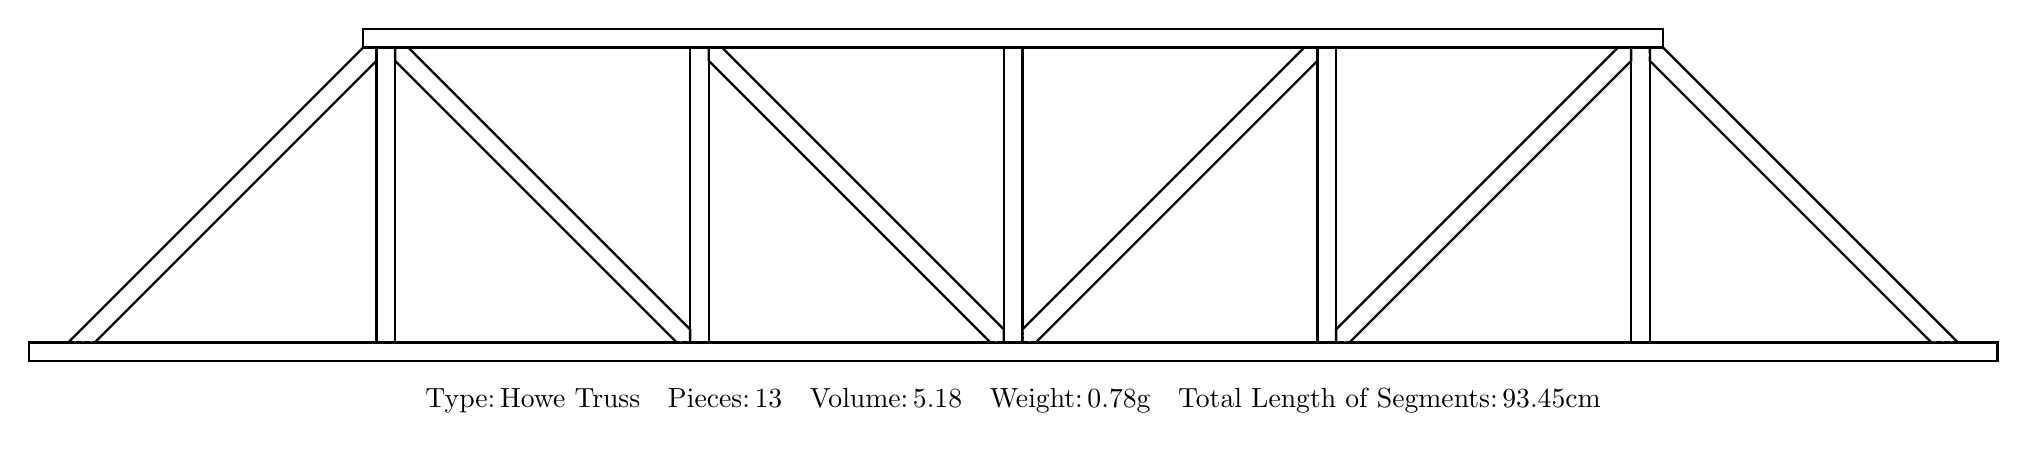
\begin{tikzpicture}
\draw[pattern=crosshatch, pattern color=white, line width=.3mm,] (-0.5,0) -- (24.5,0) -- (24.5,0.238) -- (-0.5,0.238) -- cycle;
\draw[pattern=crosshatch, pattern color=white, line width=.3mm,] (0,0.238) -- (3.74557,3.98357) -- (3.91386,3.98357) -- (3.91386,3.81528) -- (0.33658,0.238) -- cycle;
\draw[pattern=crosshatch, pattern color=white, line width=.3mm,] (24,0.238) -- (20.25443,3.98357) -- (20.08614,3.98357) -- (20.08614,3.81528) -- (23.66342,0.238) -- cycle;
\draw[pattern=crosshatch, pattern color=white, line width=.3mm,] (3.91386,0.238) -- (3.91386,3.98357) -- (4.15186,3.98357) -- (4.15186,0.238) -- cycle;
\draw[pattern=crosshatch, pattern color=white, line width=.3mm,] (7.89743,0.238) -- (7.89743,3.98357) -- (8.13543,3.98357) -- (8.13543,0.238) -- cycle;
\draw[pattern=crosshatch, pattern color=white, line width=.3mm,] (11.881,0.238) -- (11.881,3.98357) -- (12.119,3.98357) -- (12.119,0.238) -- cycle;
\draw[pattern=crosshatch, pattern color=white, line width=.3mm,] (15.86457,0.238) -- (15.86457,3.98357) -- (16.10257,3.98357) -- (16.10257,0.238) -- cycle;
\draw[pattern=crosshatch, pattern color=white, line width=.3mm,] (19.84814,0.238) -- (19.84814,3.98357) -- (20.08614,3.98357) -- (20.08614,0.238) -- cycle;
\draw[pattern=crosshatch, pattern color=white, line width=.3mm,] (12.28729,0.238) -- (15.86457,3.81528) -- (15.86457,3.98357) -- (15.69628,3.98357) -- (12.119,0.40629) -- (12.119,0.238) -- cycle;
\draw[pattern=crosshatch, pattern color=white, line width=.3mm,] (11.71271,0.238) -- (8.13543,3.81528) -- (8.13543,3.98357) -- (8.30372,3.98357) -- (11.881,0.40629) -- (11.881,0.238) -- cycle;
\draw[pattern=crosshatch, pattern color=white, line width=.3mm,] (16.27086,0.238) -- (19.84814,3.81528) -- (19.84814,3.98357) -- (19.67985,3.98357) -- (16.10257,0.40629) -- (16.10257,0.238) -- cycle;
\draw[pattern=crosshatch, pattern color=white, line width=.3mm,] (7.72914,0.238) -- (4.15186,3.81528) -- (4.15186,3.98357) -- (4.32015,3.98357) -- (7.89743,0.40629) -- (7.89743,0.238) -- cycle;
\draw[pattern=crosshatch, pattern color=white, line width=.3mm,] (3.74557,3.98357) -- (20.25443,3.98357) -- (20.25443,4.22157) -- (3.74557,4.22157) -- cycle;
\path node at (12,-0.5) {Type:\,Howe Truss\quad Pieces:\,13\quad Volume:\,5.18\quad Weight:\,0.78g\quad Total Length of Segments:\,93.45cm};
\end{tikzpicture}

	\end{figure}
	\begin{figure}
		\centering
		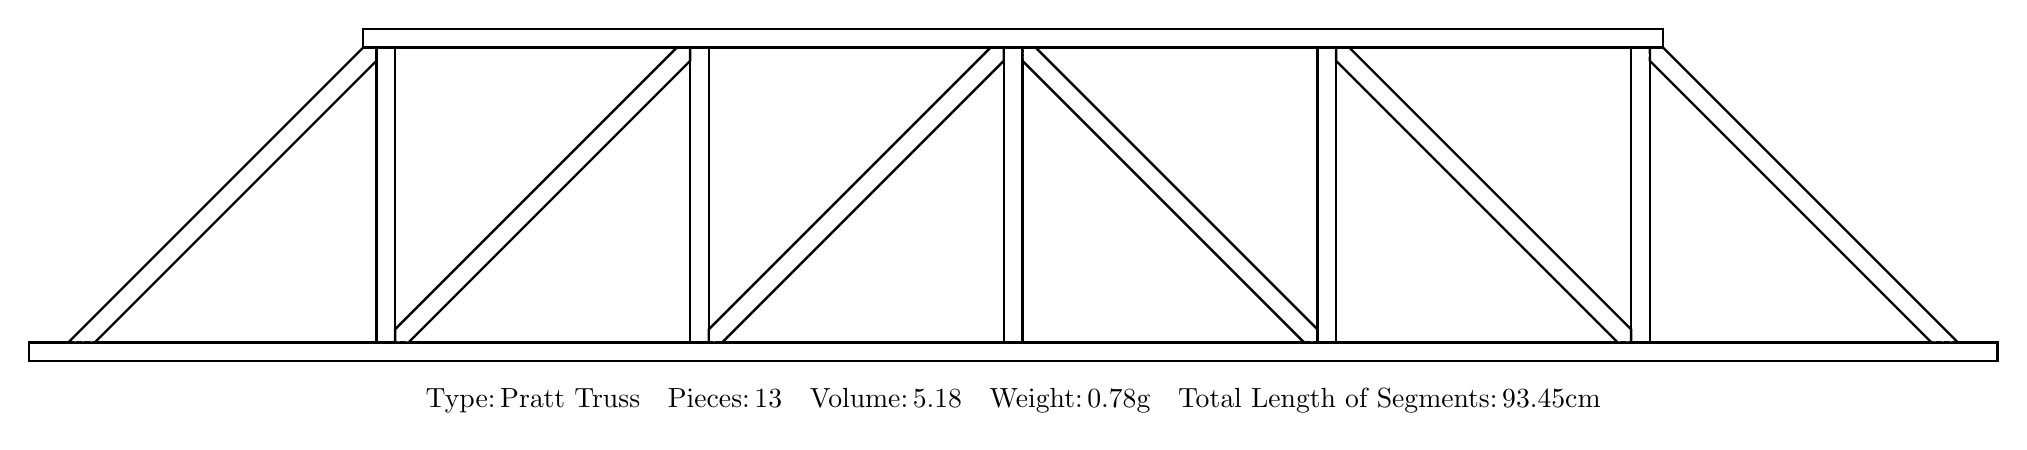
\begin{tikzpicture}
\draw[pattern=crosshatch, pattern color=white, line width=.3mm,] (-0.5,0) -- (24.5,0) -- (24.5,0.238) -- (-0.5,0.238) -- cycle;
\draw[pattern=crosshatch, pattern color=white, line width=.3mm,] (0,0.238) -- (3.74557,3.98357) -- (3.91386,3.98357) -- (3.91386,3.81528) -- (0.33658,0.238) -- cycle;
\draw[pattern=crosshatch, pattern color=white, line width=.3mm,] (24,0.238) -- (20.25443,3.98357) -- (20.08614,3.98357) -- (20.08614,3.81528) -- (23.66342,0.238) -- cycle;
\draw[pattern=crosshatch, pattern color=white, line width=.3mm,] (3.91386,0.238) -- (3.91386,3.98357) -- (4.15186,3.98357) -- (4.15186,0.238) -- cycle;
\draw[pattern=crosshatch, pattern color=white, line width=.3mm,] (7.89743,0.238) -- (7.89743,3.98357) -- (8.13543,3.98357) -- (8.13543,0.238) -- cycle;
\draw[pattern=crosshatch, pattern color=white, line width=.3mm,] (11.881,0.238) -- (11.881,3.98357) -- (12.119,3.98357) -- (12.119,0.238) -- cycle;
\draw[pattern=crosshatch, pattern color=white, line width=.3mm,] (15.86457,0.238) -- (15.86457,3.98357) -- (16.10257,3.98357) -- (16.10257,0.238) -- cycle;
\draw[pattern=crosshatch, pattern color=white, line width=.3mm,] (19.84814,0.238) -- (19.84814,3.98357) -- (20.08614,3.98357) -- (20.08614,0.238) -- cycle;
\draw[pattern=crosshatch, pattern color=white, line width=.3mm,] (4.32015,0.238) -- (7.89743,3.81528) -- (7.89743,3.98357) -- (7.72914,3.98357) -- (4.15186,0.40629) -- (4.15186,0.238) -- cycle;
\draw[pattern=crosshatch, pattern color=white, line width=.3mm,] (19.67985,0.238) -- (16.10257,3.81528) -- (16.10257,3.98357) -- (16.27086,3.98357) -- (19.84814,0.40629) -- (19.84814,0.238) -- cycle;
\draw[pattern=crosshatch, pattern color=white, line width=.3mm,] (8.30372,0.238) -- (11.881,3.81528) -- (11.881,3.98357) -- (11.71271,3.98357) -- (8.13543,0.40629) -- (8.13543,0.238) -- cycle;
\draw[pattern=crosshatch, pattern color=white, line width=.3mm,] (15.69628,0.238) -- (12.119,3.81528) -- (12.119,3.98357) -- (12.28729,3.98357) -- (15.86457,0.40629) -- (15.86457,0.238) -- cycle;
\draw[pattern=crosshatch, pattern color=white, line width=.3mm,] (3.74557,3.98357) -- (20.25443,3.98357) -- (20.25443,4.22157) -- (3.74557,4.22157) -- cycle;
\path node at (12,-0.5) {Type:\,Pratt Truss\quad Pieces:\,13\quad Volume:\,5.18\quad Weight:\,0.78g\quad Total Length of Segments:\,93.45cm};
\end{tikzpicture}

	\end{figure}
	\begin{figure}
		\centering
		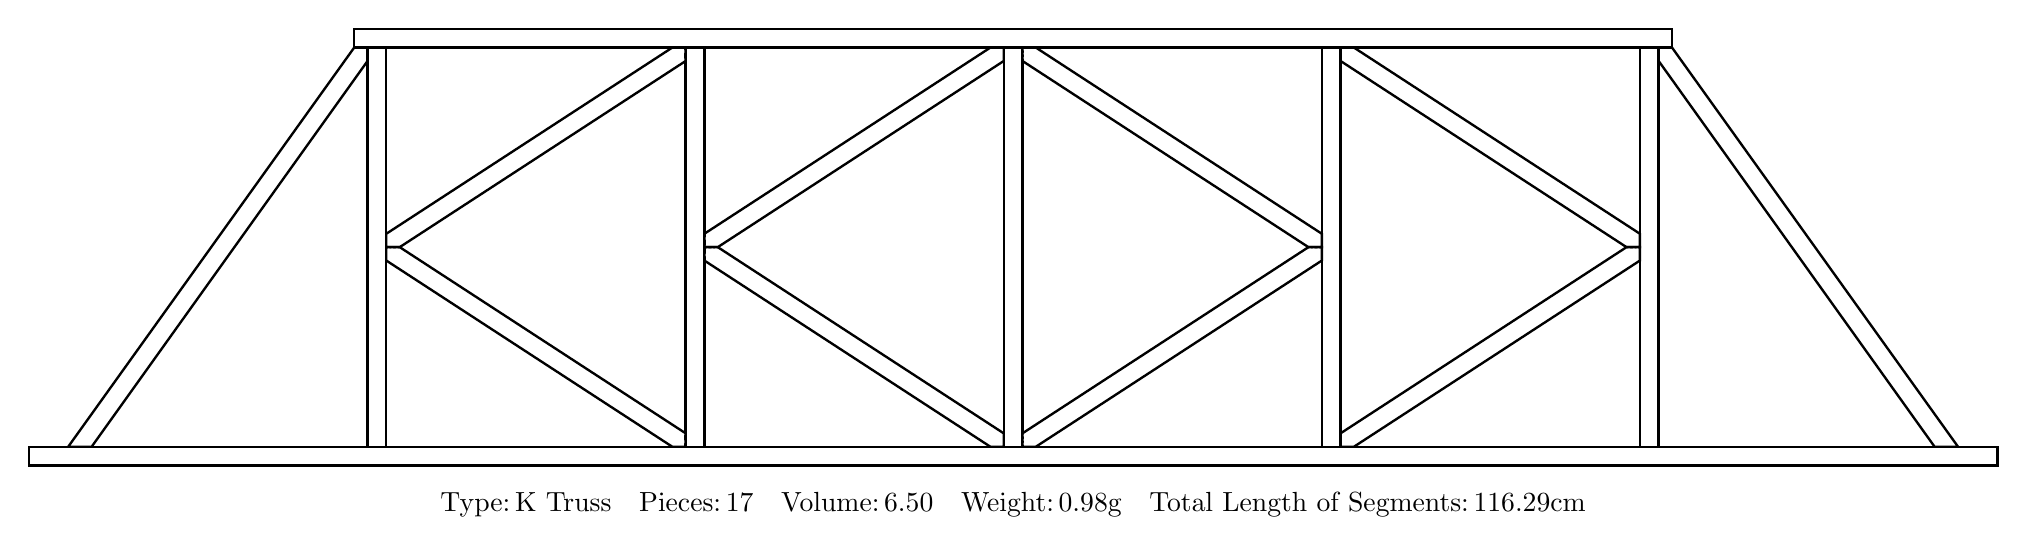
\begin{tikzpicture}
\draw[pattern=crosshatch, pattern color=white, line width=.3mm,] (-0.5,0) -- (24.5,0) -- (24.5,0.238) -- (-0.5,0.238) -- cycle;
\draw[pattern=crosshatch, pattern color=white, line width=.3mm,] (0,0.238) -- (0.2975,0.238) -- (3.80167,5.13689) -- (3.80167,5.30689) -- (3.63167,5.30689) -- cycle;
\draw[pattern=crosshatch, pattern color=white, line width=.3mm,] (24,0.238) -- (23.7025,0.238) -- (20.19833,5.13689) -- (20.19833,5.30689) -- (20.36833,5.30689) -- cycle;
\draw[pattern=crosshatch, pattern color=white, line width=.3mm,] (3.80167,0.238) -- (3.80167,5.30689) -- (4.03967,5.30689) -- (4.03967,0.238) -- cycle;
\draw[pattern=crosshatch, pattern color=white, line width=.3mm,] (7.84133,0.238) -- (7.84133,5.30689) -- (8.07933,5.30689) -- (8.07933,0.238) -- cycle;
\draw[pattern=crosshatch, pattern color=white, line width=.3mm,] (11.881,0.238) -- (11.881,5.30689) -- (12.119,5.30689) -- (12.119,0.238) -- cycle;
\draw[pattern=crosshatch, pattern color=white, line width=.3mm,] (15.92067,0.238) -- (15.92067,5.30689) -- (16.15867,5.30689) -- (16.15867,0.238) -- cycle;
\draw[pattern=crosshatch, pattern color=white, line width=.3mm,] (19.96033,0.238) -- (19.96033,5.30689) -- (20.19833,5.30689) -- (20.19833,0.238) -- cycle;
\draw[pattern=crosshatch, pattern color=white, line width=.3mm,] (4.03967,2.77244) -- (4.2098,2.77244) -- (7.84133,5.13675) -- (7.84133,5.30689) -- (7.6712,5.30689) -- (4.03967,2.94258) -- cycle;
\draw[pattern=crosshatch, pattern color=white, line width=.3mm,] (4.03967,2.77244) -- (4.03967,2.60231) -- (7.6712,0.238) -- (7.84133,0.238) -- (7.84133,0.40814) -- (4.2098,2.77244) -- cycle;
\draw[pattern=crosshatch, pattern color=white, line width=.3mm,] (8.07933,2.77244) -- (8.24947,2.77244) -- (11.881,5.13675) -- (11.881,5.30689) -- (11.71086,5.30689) -- (8.07933,2.94258) -- cycle;
\draw[pattern=crosshatch, pattern color=white, line width=.3mm,] (8.07933,2.77244) -- (8.07933,2.60231) -- (11.71086,0.238) -- (11.881,0.238) -- (11.881,0.40814) -- (8.24947,2.77244) -- cycle;
\draw[pattern=crosshatch, pattern color=white, line width=.3mm,] (19.96033,2.77244) -- (19.7902,2.77244) -- (16.15867,5.13675) -- (16.15867,5.30689) -- (16.3288,5.30689) -- (19.96033,2.94258) -- cycle;
\draw[pattern=crosshatch, pattern color=white, line width=.3mm,] (19.96033,2.77244) -- (19.96033,2.60231) -- (16.3288,0.238) -- (16.15867,0.238) -- (16.15867,0.40814) -- (19.7902,2.77244) -- cycle;
\draw[pattern=crosshatch, pattern color=white, line width=.3mm,] (15.92067,2.77244) -- (15.75053,2.77244) -- (12.119,5.13675) -- (12.119,5.30689) -- (12.28914,5.30689) -- (15.92067,2.94258) -- cycle;
\draw[pattern=crosshatch, pattern color=white, line width=.3mm,] (15.92067,2.77244) -- (15.92067,2.60231) -- (12.28914,0.238) -- (12.119,0.238) -- (12.119,0.40814) -- (15.75053,2.77244) -- cycle;
\draw[pattern=crosshatch, pattern color=white, line width=.3mm,] (3.63167,5.30689) -- (20.36833,5.30689) -- (20.36833,5.54489) -- (3.63167,5.54489) -- cycle;
\path node at (12,-0.5) {Type:\,K Truss\quad Pieces:\,17\quad Volume:\,6.50\quad Weight:\,0.98g\quad Total Length of Segments:\,116.29cm};
\end{tikzpicture}

	\end{figure}
	\begin{figure}
		\centering
		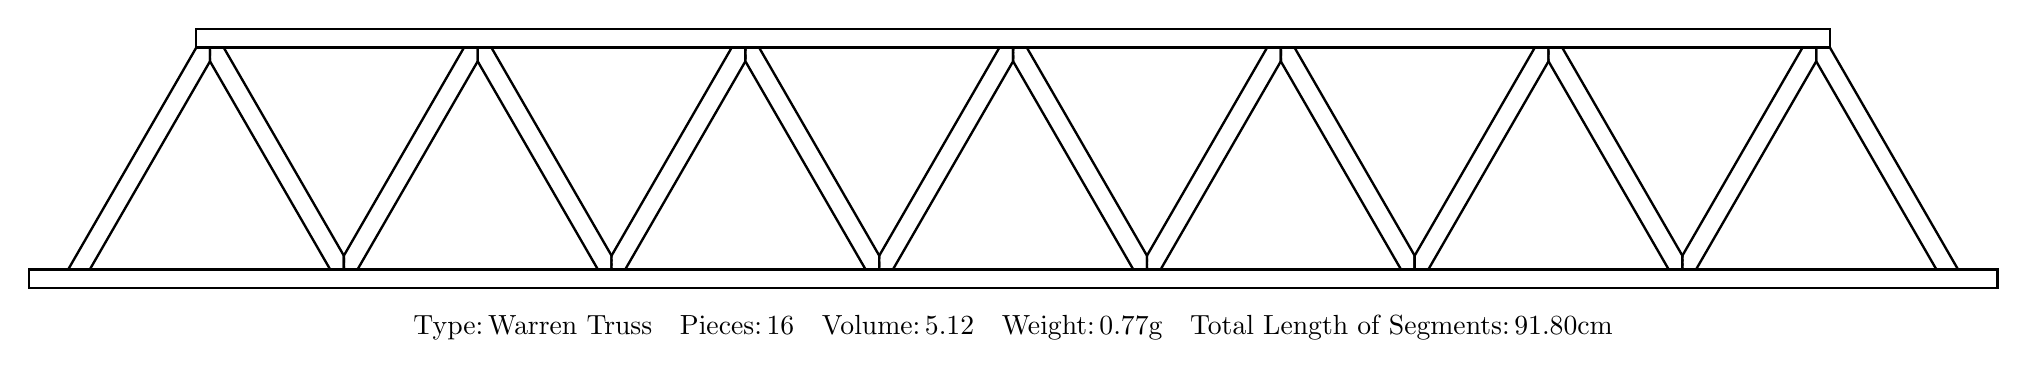
\begin{tikzpicture}
\draw[pattern=crosshatch, pattern color=white, line width=.3mm,] (-0.5,0) -- (24.5,0) -- (24.5,0.238) -- (-0.5,0.238) -- cycle;
\draw[pattern=crosshatch, pattern color=white, line width=.3mm,] (0.27482,0.238) -- (1.80051,2.88057) -- (1.80051,3.0548) -- (1.62628,3.0548) -- (0,0.238) -- cycle;
\draw[pattern=crosshatch, pattern color=white, line width=.3mm,] (23.72518,0.238) -- (22.19949,2.88057) -- (22.19949,3.0548) -- (22.37372,3.0548) -- (24,0.238) -- cycle;
\draw[pattern=crosshatch, pattern color=white, line width=.3mm,] (3.32619,0.238) -- (1.80051,2.88057) -- (1.80051,3.0548) -- (1.97473,3.0548) -- (3.50042,0.41223) -- (3.50042,0.238) -- cycle;
\draw[pattern=crosshatch, pattern color=white, line width=.3mm,] (3.67465,0.238) -- (5.20034,2.88057) -- (5.20034,3.0548) -- (5.02611,3.0548) -- (3.50042,0.41223) -- (3.50042,0.238) -- cycle;
\draw[pattern=crosshatch, pattern color=white, line width=.3mm,] (6.72603,0.238) -- (5.20034,2.88057) -- (5.20034,3.0548) -- (5.37457,3.0548) -- (6.90025,0.41223) -- (6.90025,0.238) -- cycle;
\draw[pattern=crosshatch, pattern color=white, line width=.3mm,] (7.07448,0.238) -- (8.60017,2.88057) -- (8.60017,3.0548) -- (8.42594,3.0548) -- (6.90025,0.41223) -- (6.90025,0.238) -- cycle;
\draw[pattern=crosshatch, pattern color=white, line width=.3mm,] (10.12586,0.238) -- (8.60017,2.88057) -- (8.60017,3.0548) -- (8.7744,3.0548) -- (10.30008,0.41223) -- (10.30008,0.238) -- cycle;
\draw[pattern=crosshatch, pattern color=white, line width=.3mm,] (10.47431,0.238) -- (12,2.88057) -- (12,3.0548) -- (11.82577,3.0548) -- (10.30008,0.41223) -- (10.30008,0.238) -- cycle;
\draw[pattern=crosshatch, pattern color=white, line width=.3mm,] (13.52569,0.238) -- (12,2.88057) -- (12,3.0548) -- (12.17423,3.0548) -- (13.69992,0.41223) -- (13.69992,0.238) -- cycle;
\draw[pattern=crosshatch, pattern color=white, line width=.3mm,] (13.87414,0.238) -- (15.39983,2.88057) -- (15.39983,3.0548) -- (15.2256,3.0548) -- (13.69992,0.41223) -- (13.69992,0.238) -- cycle;
\draw[pattern=crosshatch, pattern color=white, line width=.3mm,] (16.92552,0.238) -- (15.39983,2.88057) -- (15.39983,3.0548) -- (15.57406,3.0548) -- (17.09975,0.41223) -- (17.09975,0.238) -- cycle;
\draw[pattern=crosshatch, pattern color=white, line width=.3mm,] (17.27397,0.238) -- (18.79966,2.88057) -- (18.79966,3.0548) -- (18.62543,3.0548) -- (17.09975,0.41223) -- (17.09975,0.238) -- cycle;
\draw[pattern=crosshatch, pattern color=white, line width=.3mm,] (20.32535,0.238) -- (18.79966,2.88057) -- (18.79966,3.0548) -- (18.97389,3.0548) -- (20.49958,0.41223) -- (20.49958,0.238) -- cycle;
\draw[pattern=crosshatch, pattern color=white, line width=.3mm,] (20.67381,0.238) -- (22.19949,2.88057) -- (22.19949,3.0548) -- (22.02527,3.0548) -- (20.49958,0.41223) -- (20.49958,0.238) -- cycle;
\draw[pattern=crosshatch, pattern color=white, line width=.3mm,] (1.62628,3.0548) -- (22.37372,3.0548) -- (22.37372,3.2928) -- (1.62628,3.2928) -- (1.62628,3.0548) -- cycle;
\path node at (12,-0.5) {Type:\,Warren Truss\quad Pieces:\,16\quad Volume:\,5.12\quad Weight:\,0.77g\quad Total Length of Segments:\,91.80cm};
\end{tikzpicture}

	\end{figure}
	\begin{figure}
		\centering
		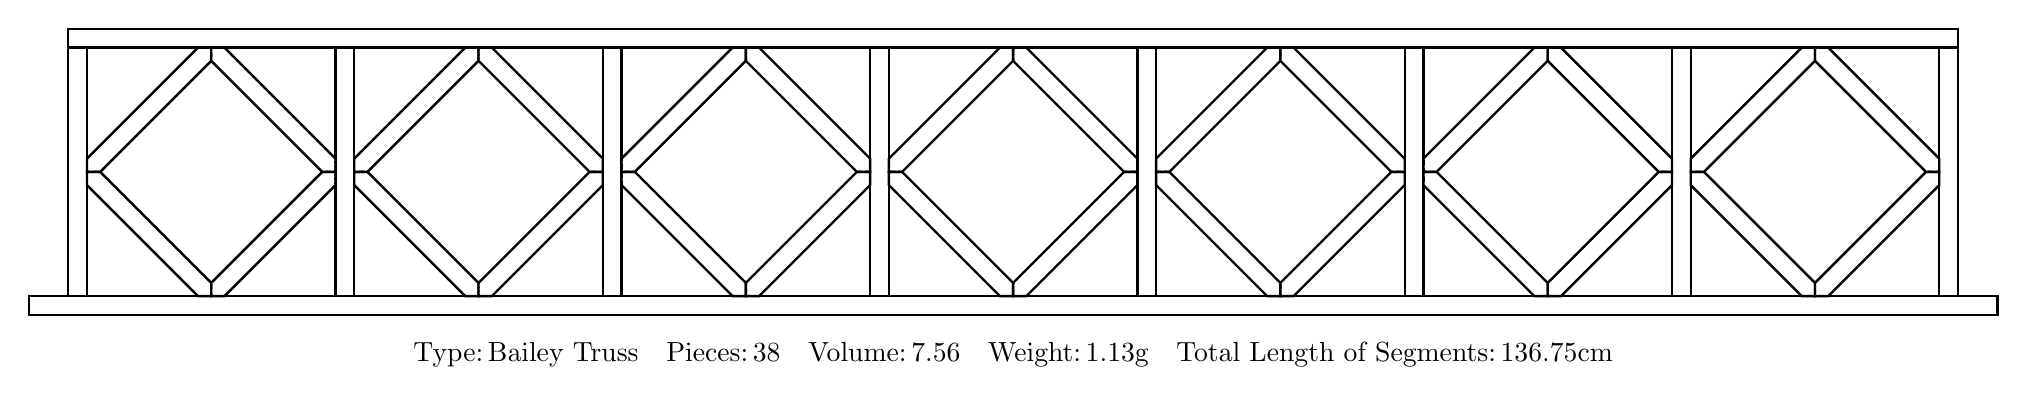
\begin{tikzpicture}
\draw[pattern=crosshatch, pattern color=white, line width=.3mm,] (-0.5,0) -- (24.5,0) -- (24.5,0.238) -- (-0.5,0.238) -- cycle;
\draw[pattern=crosshatch, pattern color=white, line width=.3mm,] (0,0.238) -- (0.238,0.238) -- (0.238,3.39457) -- (0,3.39457) -- cycle;
\draw[pattern=crosshatch, pattern color=white, line width=.3mm,] (3.39457,0.238) -- (3.63257,0.238) -- (3.63257,3.39457) -- (3.39457,3.39457) -- cycle;
\draw[pattern=crosshatch, pattern color=white, line width=.3mm,] (6.78914,0.238) -- (7.02714,0.238) -- (7.02714,3.39457) -- (6.78914,3.39457) -- cycle;
\draw[pattern=crosshatch, pattern color=white, line width=.3mm,] (10.18371,0.238) -- (10.42171,0.238) -- (10.42171,3.39457) -- (10.18371,3.39457) -- cycle;
\draw[pattern=crosshatch, pattern color=white, line width=.3mm,] (13.57829,0.238) -- (13.81629,0.238) -- (13.81629,3.39457) -- (13.57829,3.39457) -- cycle;
\draw[pattern=crosshatch, pattern color=white, line width=.3mm,] (16.97286,0.238) -- (17.21086,0.238) -- (17.21086,3.39457) -- (16.97286,3.39457) -- cycle;
\draw[pattern=crosshatch, pattern color=white, line width=.3mm,] (20.36743,0.238) -- (20.60543,0.238) -- (20.60543,3.39457) -- (20.36743,3.39457) -- cycle;
\draw[pattern=crosshatch, pattern color=white, line width=.3mm,] (23.762,0.238) -- (24,0.238) -- (24,3.39457) -- (23.762,3.39457) -- cycle;
\draw[pattern=crosshatch, pattern color=white, line width=.3mm,] (1.64799,0.238) -- (0.238,1.64799) -- (0.238,1.81629) -- (0.40629,1.81629) -- (1.81629,0.40629) -- (1.81629,0.238) -- cycle;
\draw[pattern=crosshatch, pattern color=white, line width=.3mm,] (1.98458,0.238) -- (3.39457,1.64799) -- (3.39457,1.81629) -- (3.22628,1.81629) -- (1.81629,0.40629) -- (1.81629,0.238) -- cycle;
\draw[pattern=crosshatch, pattern color=white, line width=.3mm,] (1.64799,3.39457) -- (0.238,1.98458) -- (0.238,1.81629) -- (0.40629,1.81629) -- (1.81629,3.22628) -- (1.81629,3.39457) -- cycle;
\draw[pattern=crosshatch, pattern color=white, line width=.3mm,] (1.98458,3.39457) -- (3.39457,1.98458) -- (3.39457,1.81629) -- (3.22628,1.81629) -- (1.81629,3.22628) -- (1.81629,3.39457) -- cycle;
\draw[pattern=crosshatch, pattern color=white, line width=.3mm,] (5.04257,0.238) -- (3.63257,1.64799) -- (3.63257,1.81629) -- (3.80086,1.81629) -- (5.21086,0.40629) -- (5.21086,0.238) -- cycle;
\draw[pattern=crosshatch, pattern color=white, line width=.3mm,] (5.37915,0.238) -- (6.78914,1.64799) -- (6.78914,1.81629) -- (6.62085,1.81629) -- (5.21086,0.40629) -- (5.21086,0.238) -- cycle;
\draw[pattern=crosshatch, pattern color=white, line width=.3mm,] (5.04257,3.39457) -- (3.63257,1.98458) -- (3.63257,1.81629) -- (3.80086,1.81629) -- (5.21086,3.22628) -- (5.21086,3.39457) -- cycle;
\draw[pattern=crosshatch, pattern color=white, line width=.3mm,] (5.37915,3.39457) -- (6.78914,1.98458) -- (6.78914,1.81629) -- (6.62085,1.81629) -- (5.21086,3.22628) -- (5.21086,3.39457) -- cycle;
\draw[pattern=crosshatch, pattern color=white, line width=.3mm,] (8.43714,0.238) -- (7.02714,1.64799) -- (7.02714,1.81629) -- (7.19543,1.81629) -- (8.60543,0.40629) -- (8.60543,0.238) -- cycle;
\draw[pattern=crosshatch, pattern color=white, line width=.3mm,] (8.77372,0.238) -- (10.18371,1.64799) -- (10.18371,1.81629) -- (10.01542,1.81629) -- (8.60543,0.40629) -- (8.60543,0.238) -- cycle;
\draw[pattern=crosshatch, pattern color=white, line width=.3mm,] (8.43714,3.39457) -- (7.02714,1.98458) -- (7.02714,1.81629) -- (7.19543,1.81629) -- (8.60543,3.22628) -- (8.60543,3.39457) -- cycle;
\draw[pattern=crosshatch, pattern color=white, line width=.3mm,] (8.77372,3.39457) -- (10.18371,1.98458) -- (10.18371,1.81629) -- (10.01542,1.81629) -- (8.60543,3.22628) -- (8.60543,3.39457) -- cycle;
\draw[pattern=crosshatch, pattern color=white, line width=.3mm,] (11.83171,0.238) -- (10.42171,1.64799) -- (10.42171,1.81629) -- (10.59001,1.81629) -- (12,0.40629) -- (12,0.238) -- cycle;
\draw[pattern=crosshatch, pattern color=white, line width=.3mm,] (12.16829,0.238) -- (13.57829,1.64799) -- (13.57829,1.81629) -- (13.40999,1.81629) -- (12,0.40629) -- (12,0.238) -- cycle;
\draw[pattern=crosshatch, pattern color=white, line width=.3mm,] (11.83171,3.39457) -- (10.42171,1.98458) -- (10.42171,1.81629) -- (10.59001,1.81629) -- (12,3.22628) -- (12,3.39457) -- cycle;
\draw[pattern=crosshatch, pattern color=white, line width=.3mm,] (12.16829,3.39457) -- (13.57829,1.98458) -- (13.57829,1.81629) -- (13.40999,1.81629) -- (12,3.22628) -- (12,3.39457) -- cycle;
\draw[pattern=crosshatch, pattern color=white, line width=.3mm,] (15.22628,0.238) -- (13.81629,1.64799) -- (13.81629,1.81629) -- (13.98458,1.81629) -- (15.39457,0.40629) -- (15.39457,0.238) -- cycle;
\draw[pattern=crosshatch, pattern color=white, line width=.3mm,] (15.56286,0.238) -- (16.97286,1.64799) -- (16.97286,1.81629) -- (16.80457,1.81629) -- (15.39457,0.40629) -- (15.39457,0.238) -- cycle;
\draw[pattern=crosshatch, pattern color=white, line width=.3mm,] (15.22628,3.39457) -- (13.81629,1.98458) -- (13.81629,1.81629) -- (13.98458,1.81629) -- (15.39457,3.22628) -- (15.39457,3.39457) -- cycle;
\draw[pattern=crosshatch, pattern color=white, line width=.3mm,] (15.56286,3.39457) -- (16.97286,1.98458) -- (16.97286,1.81629) -- (16.80457,1.81629) -- (15.39457,3.22628) -- (15.39457,3.39457) -- cycle;
\draw[pattern=crosshatch, pattern color=white, line width=.3mm,] (18.62085,0.238) -- (17.21086,1.64799) -- (17.21086,1.81629) -- (17.37915,1.81629) -- (18.78914,0.40629) -- (18.78914,0.238) -- cycle;
\draw[pattern=crosshatch, pattern color=white, line width=.3mm,] (18.95743,0.238) -- (20.36743,1.64799) -- (20.36743,1.81629) -- (20.19914,1.81629) -- (18.78914,0.40629) -- (18.78914,0.238) -- cycle;
\draw[pattern=crosshatch, pattern color=white, line width=.3mm,] (18.62085,3.39457) -- (17.21086,1.98458) -- (17.21086,1.81629) -- (17.37915,1.81629) -- (18.78914,3.22628) -- (18.78914,3.39457) -- cycle;
\draw[pattern=crosshatch, pattern color=white, line width=.3mm,] (18.95743,3.39457) -- (20.36743,1.98458) -- (20.36743,1.81629) -- (20.19914,1.81629) -- (18.78914,3.22628) -- (18.78914,3.39457) -- cycle;
\draw[pattern=crosshatch, pattern color=white, line width=.3mm,] (22.01542,0.238) -- (20.60543,1.64799) -- (20.60543,1.81629) -- (20.77372,1.81629) -- (22.18371,0.40629) -- (22.18371,0.238) -- cycle;
\draw[pattern=crosshatch, pattern color=white, line width=.3mm,] (22.35201,0.238) -- (23.762,1.64799) -- (23.762,1.81629) -- (23.59371,1.81629) -- (22.18371,0.40629) -- (22.18371,0.238) -- cycle;
\draw[pattern=crosshatch, pattern color=white, line width=.3mm,] (22.01542,3.39457) -- (20.60543,1.98458) -- (20.60543,1.81629) -- (20.77372,1.81629) -- (22.18371,3.22628) -- (22.18371,3.39457) -- cycle;
\draw[pattern=crosshatch, pattern color=white, line width=.3mm,] (22.35201,3.39457) -- (23.762,1.98458) -- (23.762,1.81629) -- (23.59371,1.81629) -- (22.18371,3.22628) -- (22.18371,3.39457) -- cycle;
\draw[pattern=crosshatch, pattern color=white, line width=.3mm,] (0,3.39457) -- (24,3.39457) -- (24,3.63257) -- (0,3.63257) -- (0,3.39457) -- cycle;
\path node at (12,-0.5) {Type:\,Bailey Truss\quad Pieces:\,38\quad Volume:\,7.56\quad Weight:\,1.13g\quad Total Length of Segments:\,136.75cm};
\end{tikzpicture}

	\end{figure}
\end{document}